% =====================================================================
% Rozdział 4 – Projekt systemu (WZÓR, ok. 4,5 strony)
% Styl bezosobowy. Rysunki: rysunki/znacznik_pi_wymiary.pdf, rysunki/baza_erd.pdf (6 tabel, wersja 28.10),
% rysunki/diagram_klas.pdf (wersja 28.10); zrzut ekranu aplikacji – do wykonania (TODO poniżej).
% Plan i zwroty: materialy/06_plan_zwroty_rozdzialy_4_7.md.
% Wymaga pakietów: booktabs, tabularx.
% =====================================================================

\chapter{Projekt systemu}
\label{chap:projekt}

W rozdziale opisano decyzje projektowe, które pozwalają spełnić wymagania przedstawione w rozdziale~\ref{chap:analiza}: dobór technologii, projekt znacznika referencyjnego, bazy danych, struktury klas oraz interfejsu użytkownika.

\section{Dobór technologii}
\label{sec:technologie}

Przy wyborze technologii kierowano się dostępnością gotowych implementacji metod opisanych w rozdziale~\ref{chap:stan-wiedzy}, możliwością pracy bez procesora graficznego oraz prostotą instalacji na komputerze użytkownika. Wykorzystane technologie zestawiono w tabeli~\ref{tab:technologie}.

\begin{table}[htbp]
  \centering
  \caption{Technologie wykorzystane w systemie}
  \label{tab:technologie}
  \small
  \begin{tabularx}{\textwidth}{>{\raggedright\arraybackslash}p{3.0cm} >{\raggedright\arraybackslash}p{3.3cm} X}
    \toprule
    Element & Technologia & Uzasadnienie \\
    \midrule
    język programowania & Python 3.14 (aplikacja) & bogaty ekosystem bibliotek przetwarzania obrazów i uczenia maszynowego; jeden język dla aplikacji i modeli \\
    przetwarzanie obrazów i rejestracja & OpenCV 4.13, NumPy 2.4 & gotowa implementacja kryterium ECC~\cite{evangelidis2008}, operacji morfologicznych i wnioskowania sieci w formacie ONNX \\
    uczenie głębokie & PyTorch 2.11 (osobne środowisko, Python 3.12) & trening sieci U-Net i douczanie modelu PanDerm, którego wagi udostępniono dla tej biblioteki \\
    wnioskowanie sieci U-Net & ONNX + moduł \texttt{dnn} biblioteki OpenCV & uruchamianie modelu bez biblioteki PyTorch (WN7) \\
    interfejs graficzny & customtkinter 5.2 (nakładka na tkinter) & lekka biblioteka o otwartej licencji; tkinter jest częścią instalacji Pythona \\
    baza danych & SQLite & baza w jednym pliku, niewymagająca serwera, wystarczająca dla jednego użytkownika \\
    odczyt nagrań termowizyjnych & flirpy 0.3 & klatki i surowe wartości detektora z nagrań .SEQ kamery FLIR A320 (WF15) \\
    adnotacje & CVAT & oznaczanie masek i punktów (narożników) w przeglądarce \\
    raport & HTML, JSON, PNG & raport czytelny bez dodatkowego oprogramowania; wyniki w formacie do dalszej analizy \\
    metoda porównawcza & SimpleITK 2.5 & rejestracja z informacją wzajemną~\cite{zitova2003} w badaniu porównawczym \\
    \bottomrule
  \end{tabularx}
\end{table}

Rozważano także rejestrację bezpośrednio na intensywnościach obu obrazów z użyciem informacji wzajemnej~\cite{zitova2003,correlation-ratio} (metryka \texttt{MattesMutualInformation} biblioteki SimpleITK). Podejście to zastosowano we wcześniejszej wersji systemu i zachowano jako metodę porównawczą, natomiast w systemie docelowym transformację wyznacza się na maskach znacznika, zgodnie z wnioskami z przeglądu literatury (podrozdział~\ref{sec:modele-transformacji}). Zrezygnowano również z przechowywania wyników w plikach CSV na rzecz bazy danych, która zachowuje historię analiz i relacje między danymi.

\section{Projekt znacznika referencyjnego}
\label{sec:znacznik}

Znacznik referencyjny powinien spełniać następujące wymagania: być widoczny zarówno na zdjęciu, jak i na obrazie termowizyjnym; mieć kształt pozwalający jednoznacznie wyznaczyć położenie, skalę i kąt obrotu; zawierać punkty charakterystyczne umożliwiające wyznaczenie skali w milimetrach i ocenę błędu rejestracji; pozostawiać miejsce na znamię oraz być tani i łatwy do naklejenia.

Znacznik wykonano z taśmy pokrytej folią aluminiową. Na zdjęciu folia jest szara, o metalicznym połysku i teksturze załamań, a na obrazie termowizyjnym wyraźnie różni się od skóry, której emisyjność jest bliska jedności~\cite{infared-thermal-imaging}. Element aluminiowy (schłodzoną płytę) jako źródło kontrastu w obrazie termowizyjnym wykorzystano także w~\cite{gonzalezperez2021}.

Znacznik ma kształt litery $\Pi$ o wymiarach 35~$\times$~26~mm i szerokości paska 9~mm (rys.~\ref{fig:znacznik}). Otwór między ramionami ma wymiary 17~$\times$~17~mm (pole 289~mm$^2$) i wyznacza obszar zainteresowania, w którym umieszcza się znamię. Osiem narożników znacznika (P1--P8) służy do wyznaczenia homografii przekształcającej piksele na milimetry oraz do oceny błędu rejestracji. Kształt nie ma symetrii obrotowej, dzięki czemu kąt obrotu jest wyznaczany jednoznacznie w pełnym zakresie 360°. Znacznik jest jednak symetryczny względem osi pionowej, więc odbicie lustrzane obrazu dałoby fałszywe dopasowanie z zamienionymi ramionami; ponieważ żadna z kamer nie odwraca obrazu, przypadku tego nie rozpatruje się.

\begin{figure}[htbp]
  \centering
  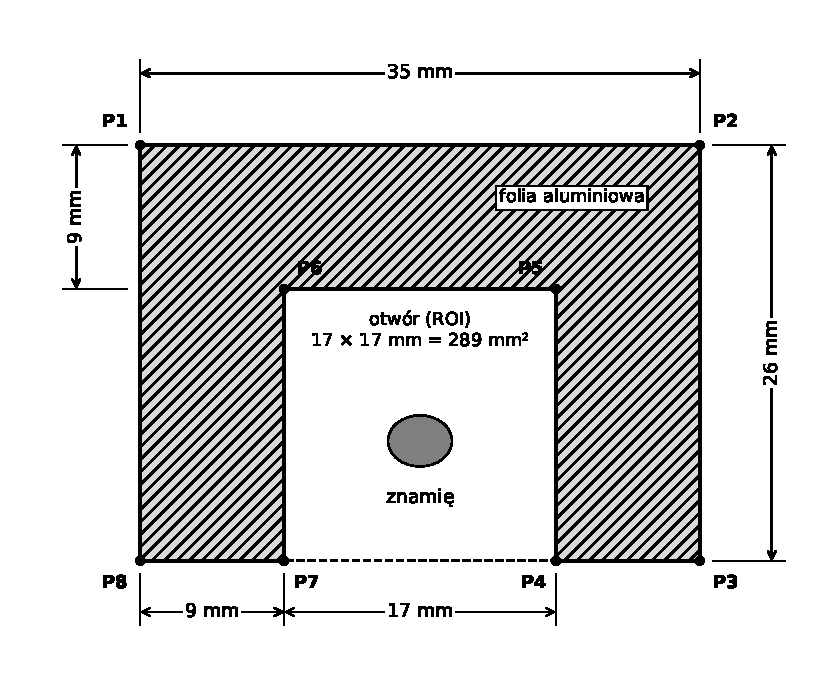
\includegraphics[width=0.6\textwidth]{rysunki/znacznik_pi_wymiary.pdf}
  \caption{Wymiary znacznika referencyjnego $\Pi$; P1--P8 -- narożniki wykorzystywane do wyznaczenia skali i błędu rejestracji}
  \label{fig:znacznik}
\end{figure}

We wcześniejszej wersji systemu stosowano znaczniki o dowolnym kształcie, bez wyróżnionych punktów, co uniemożliwiało wyznaczenie skali w milimetrach i niezależną ocenę dokładności rejestracji. Znany kształt znacznika $\Pi$ pozwala natomiast porównywać wykryte maski ze wzorcem i ostrzegać o niepewnej detekcji.

\section{Projekt bazy danych}
\label{sec:baza}

Baza danych przechowuje informacje o zbiorze (znamiona, pary obrazów, adnotacje) oraz wyniki wszystkich analiz. Pliki obrazów, masek i raportów pozostają w folderach, a baza zawiera ich ścieżki względne. Rozwiązanie to ogranicza rozmiar bazy i pozwala przeglądać pliki bez dodatkowych narzędzi. Model danych przedstawiono na diagramie związków encji (rys.~\ref{fig:erd}), a opis tabel -- w tabeli~\ref{tab:baza}.

\begin{figure}[htbp]
  \centering
  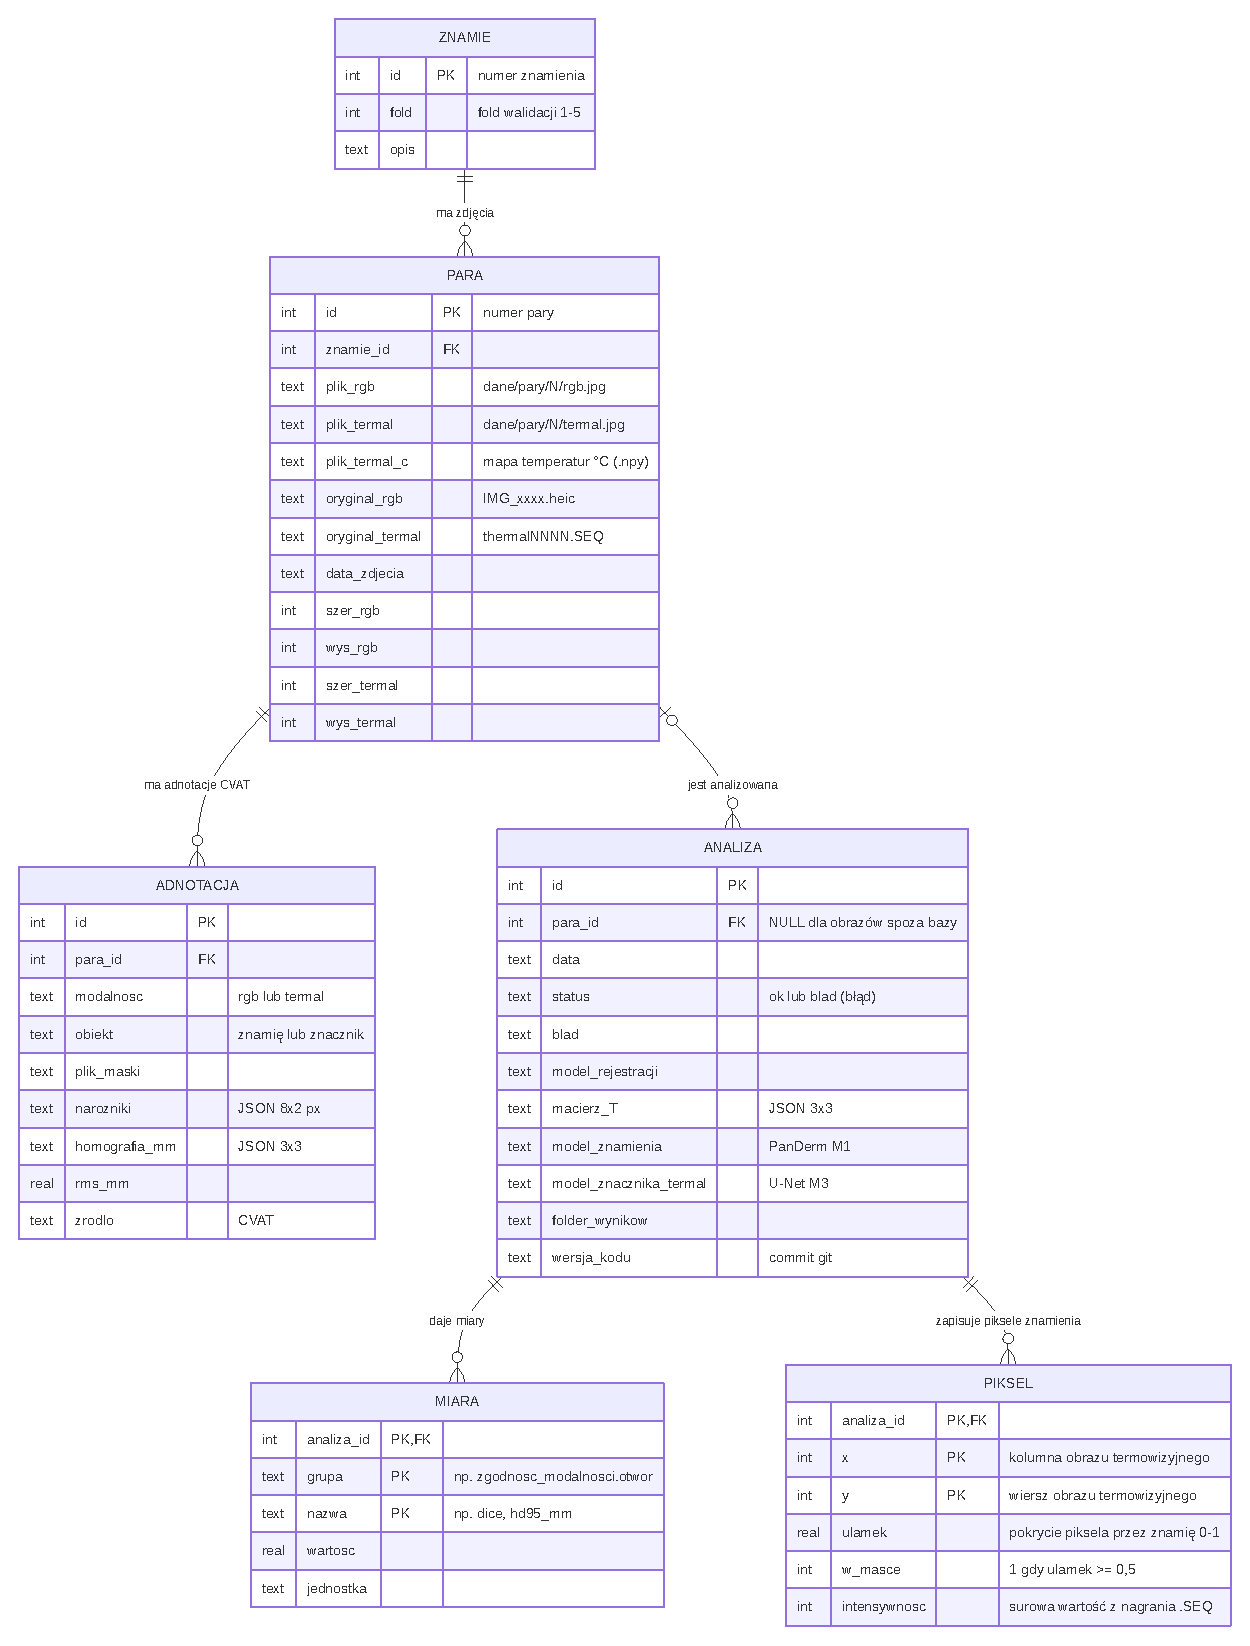
\includegraphics[width=0.62\textwidth]{rysunki/baza_erd.pdf}
  \caption{Diagram związków encji bazy danych systemu}
  \label{fig:erd}
\end{figure}

\begin{table}[htbp]
  \centering
  \caption{Tabele bazy danych}
  \label{tab:baza}
  \small
  \begin{tabularx}{\textwidth}{l X}
    \toprule
    Tabela & Zawartość \\
    \midrule
    \texttt{znamie} & numer znamienia i numer foldu walidacji krzyżowej \\
    \texttt{para} & ścieżki zdjęcia i obrazu termowizyjnego, nazwy plików oryginalnych, data wykonania zdjęcia, rozdzielczości; klucz obcy do tabeli \texttt{znamie} \\
    \texttt{adnotacja} & maski i narożniki znacznika z programu CVAT oraz homografia piksele--milimetry dla danej modalności \\
    \texttt{analiza} & każde uruchomienie analizy: data, status, użyte modele, macierz $T$, folder wyników i wersja kodu \\
    \texttt{miara} & wszystkie wyniki liczbowe analizy w postaci: grupa, nazwa, wartość, jednostka \\
    \texttt{piksel} & piksele obrazu termowizyjnego objęte znamieniem przeniesionym ze zdjęcia: współrzędne $x$, $y$, ułamek pokrycia, przynależność do maski i surowa intensywność z nagrania \\
    \bottomrule
  \end{tabularx}
\end{table}

Tabele połączono relacjami jeden do wielu: znamię ma wiele par obrazów, para -- wiele adnotacji i analiz, a analiza -- wiele miar i wiele pikseli znamienia. Tabelę \texttt{miara} zaprojektowano w układzie „długim” (jedna wartość w wierszu), dzięki czemu dodanie nowej miary nie wymaga zmiany schematu bazy. Dodatkowo zdefiniowano dwa widoki: \texttt{ostatnia\_analiza}, wskazujący najnowszą udaną analizę każdej pary, oraz \texttt{wyniki\_par}, łączący jej miary z numerem znamienia i foldu. Tabela \texttt{piksel} ma klucz główny złożony z identyfikatora analizy i współrzędnych piksela, co wyklucza powtórzenie piksela w jednej analizie i pozwala pobrać piksele znamienia jednym zapytaniem (WF15). Schemat bazy ma numer wersji; przy otwarciu bazy w starszej wersji brakujące tabele są tworzone automatycznie, bez utraty zapisanych analiz. Zapis do bazy następuje automatycznie po wygenerowaniu raportu (WF12, WN9).

\section{Diagram klas}
\label{sec:klasy}

Strukturę statyczną systemu przedstawiono na diagramie klas (rys.~\ref{fig:klasy}). Dla czytelności pominięto metody pomocnicze. Centralną klasą systemu jest \texttt{Analiza}, która przechowuje stan analizy jednej pary obrazów -- obrazy, macierz $T$, maski, narożniki, surowe wartości detektora, piksele znamienia i wyniki -- a jej metody odpowiadają kolejnym etapom potoku przetwarzania. Klasa \texttt{Aplikacja} realizuje interfejs graficzny i korzysta z obiektu klasy \texttt{Analiza}; podglądy obrazów realizuje klasa \texttt{Podglad}. Zapis wyników zapewnia klasa \texttt{Baza}, a niepowodzenia etapów są zgłaszane wyjątkiem \texttt{BladEtapu}, którego treść jest wyświetlana użytkownikowi (WN6).

\begin{figure}[htbp]
  \centering
  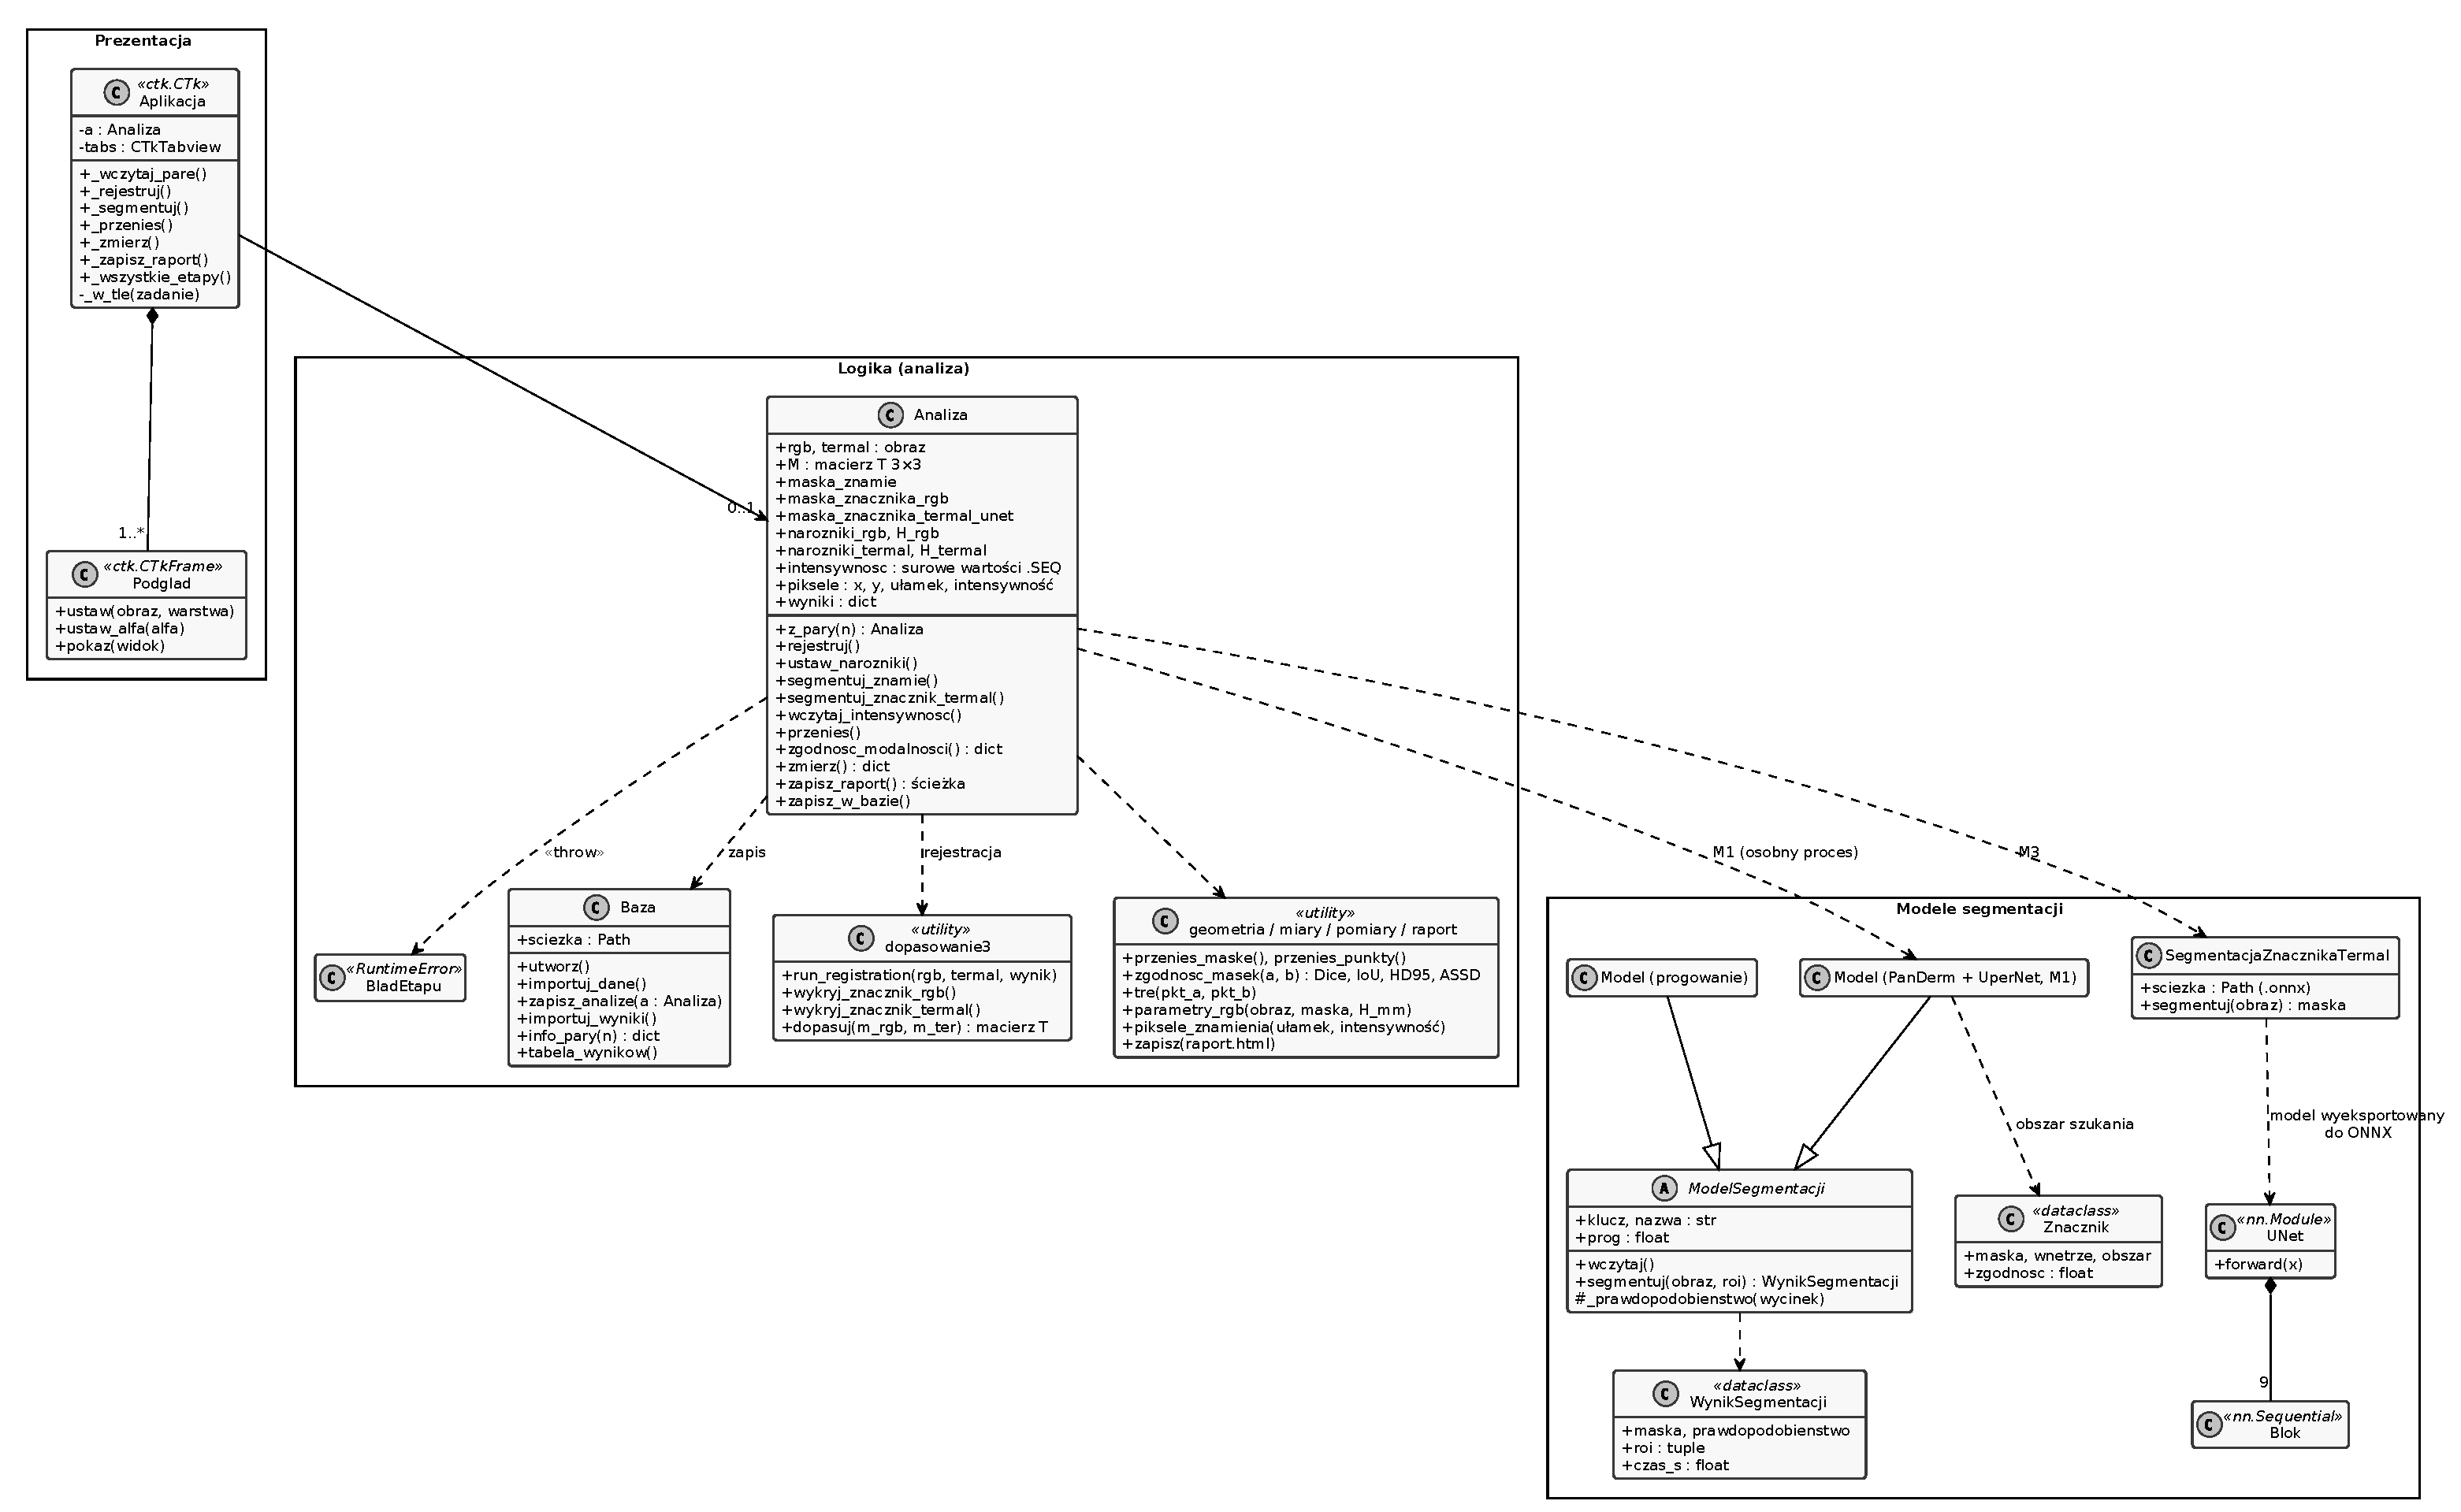
\includegraphics[width=\textwidth]{rysunki/diagram_klas.pdf}
  \caption{Diagram klas systemu (z pominięciem metod pomocniczych)}
  \label{fig:klasy}
\end{figure}

Modele segmentacji zdjęć dziedziczą po klasie abstrakcyjnej \texttt{ModelSegmentacji}, która definiuje wspólny interfejs wczytania modelu i segmentacji. Pozwala to dodawać kolejne modele bez zmiany pozostałych części systemu. Segmentację znacznika na obrazie termowizyjnym realizuje klasa \texttt{SegmentacjaZnacznikaTermal}, wykorzystująca sieć \texttt{UNet} wyeksportowaną do formatu ONNX. Moduły realizujące rejestrację, przekształcenia geometryczne, miary i raport zaimplementowano jako zbiory funkcji, oznaczone na diagramie stereotypem \guillemotleft utility\guillemotright.

\section{Projekt interfejsu użytkownika}
\label{sec:interfejs}

Interfejs zaprojektowano tak, aby odzwierciedlał kolejność etapów przetwarzania. Okno aplikacji składa się z czterech obszarów (rys.~\ref{fig:interfejs}): paska sześciu etapów (Dane, Rejestracja, Segmentacja, Przeniesienie ROI, Pomiary, Raport), panelu sterowania po lewej stronie, podglądów obrazów po prawej oraz paska stanu z dziennikiem zdarzeń w dolnej części okna.

\begin{figure}[htbp]
  \centering
  % TODO: wstawić zrzut ekranu zakładki „2. Rejestracja” (para 14) z oznaczonymi obszarami 1–4:
  % \includegraphics[width=\textwidth]{rysunki/interfejs_rejestracja.png}
  \fbox{\parbox[c][5cm][c]{0.9\textwidth}{\centering Zrzut ekranu aplikacji -- do wstawienia}}
  \caption{Okno aplikacji -- zakładka rejestracji: 1~--~pasek etapów, 2~--~panel sterowania, 3~--~podgląd nałożenia obrazów, 4~--~pasek stanu i dziennik zdarzeń}
  \label{fig:interfejs}
\end{figure}

Każda zakładka kończy się przyciskiem przejścia do kolejnego etapu, a przyciski etapów, których nie można jeszcze wykonać, są nieaktywne, co zapobiega uruchomieniu etapu bez wyników poprzedniego. Podglądy obrazów umożliwiają powiększanie (kółko myszy), przesuwanie (przeciąganie) i powrót do widoku początkowego (dwukrotne kliknięcie), a nałożenie obrazów ma regulowaną przezroczystość (WF3). Obliczenia są wykonywane w osobnym wątku, dzięki czemu interfejs pozostaje responsywny, a postęp jest widoczny na pasku stanu i w dzienniku (WN3). W zakładce pomiarów wybranie nazwy wielkości wyświetla jej objaśnienie, a w zakładce raportu można przejrzeć obrazy raportu, w tym piksele znamienia na obrazie termowizyjnym. Dane można wczytać na dwa sposoby: wybierając numer pary ze zbioru albo dwa dowolne pliki (WF1); dostępne jest też polecenie wykonania wszystkich etapów (WF13). Szczegółowy opis obsługi zawiera instrukcja użytkownika (Dodatek~A).
